\documentclass[10pt,a4paper]{article}
\usepackage[margin=2.2cm]{geometry}
\usepackage{fontspec}
\usepackage{kotex}
\setmainfont{Apple SD Gothic Neo}
\setsansfont{Apple SD Gothic Neo}
\usepackage{amsmath,amssymb}
\usepackage{graphicx}
\usepackage{booktabs}
\usepackage{caption}
\usepackage[dvipsnames]{xcolor}
\usepackage[colorlinks=true,linkcolor=MidnightBlue,citecolor=MidnightBlue,
            urlcolor=MidnightBlue]{hyperref}
\usepackage{titlesec}
\titleformat{\section}{\large\bfseries}{\thesection}{0.6em}{}
\titleformat{\subsection}{\normalsize\bfseries}{\thesubsection}{0.5em}{}
\captionsetup{font=small,labelfont=bf}
\setlength{\parskip}{0.35em}
\setlength{\parindent}{0pt}

\usepackage{mdframed}
\newmdenv[linewidth=0.4pt,linecolor=gray!60,backgroundcolor=gray!5,
          innertopmargin=6pt,innerbottommargin=6pt,skipabove=8pt,skipbelow=8pt]{claimbox}
\newcommand{\claim}[2]{\begin{claimbox}\textbf{주장.} #1\par\smallskip
  \textcolor{gray!70}{\textbf{반증 조건.} #2}\end{claimbox}}

\title{\bfseries 드리프트는 예고돼 있었다\\[2pt]
\large 학습 안의 옮김이 학습 밖의 옮김을 가리킨다}
\author{월드모델 실험실 · 노트 $800$}
\date{2026-08-07}
\begin{document}\maketitle

\section{한 줄}

절대값 이야기의 세 걸음째다. 논문 $159$(노트 $791$)가 \textbf{실패의 $86\%$ 는
드리프트}임을 쟀고, 그 상쇄는 \textbf{전이적}(유보 분포가 필요 · 배치 채점 전용)
이었다. 남은 물음: \emph{드리프트를 학습만으로 미리 알 수 있나?}

\textbf{알 수 있다.} T$=2023$ 으로 적합해 \textbf{학습 안에서} 잰 옮김(안 옮김)이,
T$=2025$ 챔피언의 \textbf{학습$\to$유보} 옮김(밖 옮김)을 가리킨다 ---
스피어만 $\mathbf{r = 0.762}$(씨앗 셋 \textbf{동일}) · 부호 $8/8$ · $n=8$.
사전등록 문턱($r \geq 0.75$ · 부호 $\geq 7/8$)을 넘어 \textbf{판정 (가)}다.

\textbf{그리고 여기서 멈춘다} --- 보정은 다음 사이클에 새로 사전등록한다
(노트 $133$ · 사전등록에 미리 적어 둔 절차다).

\begin{figure}[t]\centering
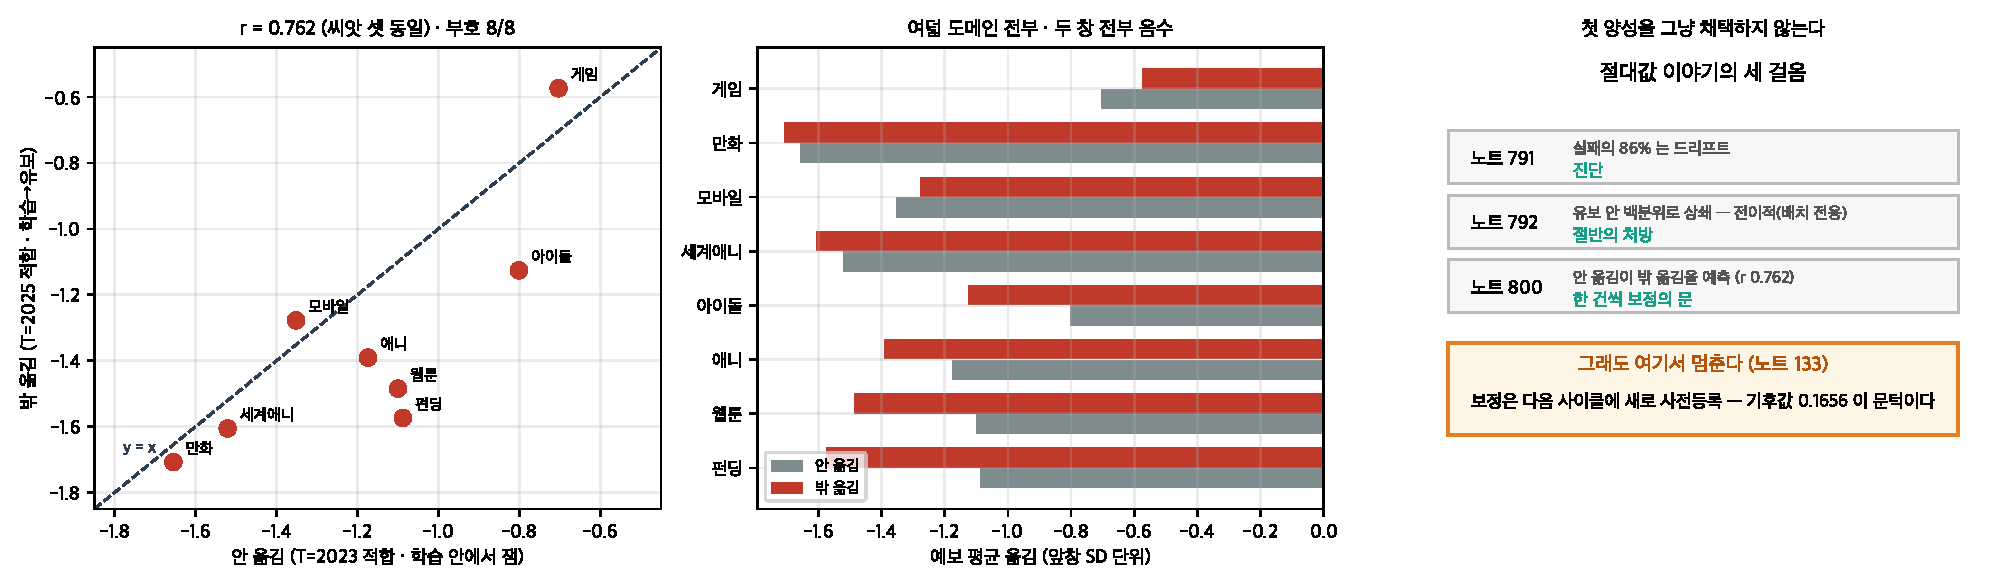
\includegraphics[width=0.99\textwidth]{figs/drift.pdf}
\caption{왼쪽: 안 옮김 대 밖 옮김 --- $y{=}x$ 근처에 선다. 가운데: \textbf{여덟
도메인 전부, 두 창 전부 음수.} 오른쪽: 세 걸음과 멈추는 자리.}
\end{figure}

\section{측정}

안 옮김 $=$ (2023{\textasciitilde}24행 예보 평균 $-$ 2023 이전행 예보 평균) $/$
SD(이전행 예보), \textbf{T$=2023$ 적합으로} --- 즉 이 수는 \textbf{2025 유보를 한
번도 안 본다.} 밖 옮김은 노트 $791$ 정의 그대로. 두 적합 모두에서 학습 안에 있는
도메인만 잰다($8$개 · 뺀 것: 도서 행 부족 · 시장팝업·팝업 훈련 밖).

\begin{center}
\begin{tabular}{lrr}
\toprule
& 안 옮김 & 밖 옮김 \\
\midrule
만화 & $-1.655$ & $-1.708$ \\
모바일 & $-1.352$ & $-1.278$ \\
세계애니 & $-1.521$ & $-1.606$ \\
게임 & $-0.703$ & $-0.573$ \\
웹툰 & $-1.100$ & $-1.485$ \\
펀딩 & $-1.088$ & $-1.574$ \\
\bottomrule
\end{tabular}
\end{center}

라벨 옮김은 $6/8$ 에서 $|x| < 0.5$ --- \textbf{옮기는 것은 예보지 라벨이 아니라는}
노트 $791$ 의 관찰이 재현된다.

\claim{\textbf{드리프트는 경계 사건이 아니라 연속 현상이다.} 내 사전 예측은
(나) $55\%$ 였다 --- \emph{``2023 경계와 2025 경계는 다른 사건이라 안
이어진다''}. \textbf{틀렸다.} 여덟 도메인이 두 창 모두 음수로, 예보는
\textbf{새 행일수록 눌린다.} 자료 구성 변화가 아니라 \textbf{시간 축 자체의
성질}로 읽힌다 --- 챔피언의 시간 입력이 $\log_{10}$(경과일수)라 새 작품은
경과일이 짧아 예보가 눌리는 구조가 기제 후보다(안 갈랐다 --- 보정 사이클에서
같이 본다).}
{\textbf{부호 $8/8$ 은 보기보다 약하다} --- 드리프트가 보편적이면 부호 일치는
자동이다. 진짜 정보는 \textbf{크기의 순위 상관 $0.762$} 이고 그것이 문턱
$0.75$ 를 \textbf{간신히} 넘는다($n{=}8$). 그리고 웹툰($-1.10 \to -1.49$)과
펀딩($-1.09 \to -1.57$)은 밖이 더 크다 --- \textbf{안 옮김은 하한쪽 추정이라
보정이 모자랄 수 있다.}}

\section{무엇이 열렸고 어디서 멈추나}

노트 $792$ 의 상쇄는 유보 예보의 \emph{분포}가 필요해서 \textbf{한 건씩 예보에
못 쓴다.} 안 옮김은 \textbf{학습에서만 나오므로} 그 제약이 없다 --- 도메인별로
유보 예보 평균을 미리 미는 보정이 이론상 선다.

\claim{\textbf{다음 사이클의 사전등록을 지금 적어 뒀다}(T$6$ 미결 ① · 네 갈래 ·
규약 $45$): 보정 후 자릿수 오차가 \textbf{기후값 $0.1656$} 보다 씨앗 SD $3$배
이상 낮아야 (가)이고, 전이적 상쇄의 $0.1880$ 과도 견준다. \textbf{r $0.762$ 가
보정의 성공을 보장하지 않는다} --- 순위가 이어지는 것과 크기가 맞는 것은 다른
일이고, $792$ 에서 드리프트를 \emph{완전히} 상쇄해도 기후값과 비겼다.}
{정직한 상한: \textbf{이 길의 최선이 $0.1880$ 근처라면}(전이적 상쇄가 그 값이다)
\textbf{보정은 기후값을 못 이긴다.} 이 실험의 진짜 값은 능력이 아니라
\textbf{기제}(시간 축이 드리프트를 만든다)일 수 있고, 그러면 고칠 곳은 보정
층이 아니라 \textbf{정식화의 시간 입력}이다 --- 그것은 판 $\rho$ 를 흔드는
일이라 채택 규약 전체를 통과해야 한다.}

\end{document}
